\documentclass[sigconf,screen,9pt]{acmart}

% Flag to disable all editing macros and make the document ready for
%  submission.
\newif\ifEditMode

% Editing mode.
\EditModetrue
% % Submission mode.
% % The `submission' mode merges certain comments and edits, and removes some
% % other notes, TODOs and remarks. For more details, refer to the `reviewing
% % macros' in the `vusec.sty' file.
% \EditModefalse


\usepackage{vu}
\usepackage{frontmatter}
\usepackage{aliases}
\usepackage{algorithm} 
\usepackage{algpseudocode} 
\usepackage{bbm}
\usepackage{amsmath}

\begin{document}






%% Thesis title.
\newcommand{\thesistitle}{Literature Study: Integrating SQL/PGQ in DuckDB}


%% Author information.
%% (Used in a couple of places, so it's better to define them in one place.)
\newcommand{\thauthor}{Daniël ten Wolde}
\newcommand{\thauthorid}{2619049}
\newcommand{\thauthoremail}{d.l.j.ten.wolde@student.vu.nl}
\newcommand{\thauthoraff}{Vrije Universiteit Amsterdam}


%% Thesis type.
%% Valid values are `vubachelor', `csmaster', `pdcsmaster', and `litstudy'.
%%
% \thtype{csmaster}

%% Thesis title.
\thtitle{\thesistitle}

%% Paper/thesis author.
\thauthname{\thauthor}

%% First supervisor.
% \thsvfirst{Peter Boncz}{First supervisor's title}

%% Daily supervisor.
% \thsvdaily{Daily supervisor's name}{Daily supervisor's title}

%% Second reader.
% \thrdrsecond{Second reader's name}{Second reader's title}

%% Attach customize front matter.
\addfrontmatter{}


\title{\thesistitle}

\author{\thauthor}
\affiliation{
  \institution{\thauthoraff}
  \city{Amsterdam}
  \country{The Netherlands}
}
\email{\thauthoremail}


% \begin{abstract}
% This thesis will focus on implementing path finding algorithms in the open-source in-process SQL OLAP database management system DuckDB. This is done to further complete the integration of SQL/PGQ, an extension of SQL, in DuckDB. 
The algorithms, one of which is a batched version of Bellman-Ford, will make it possible to retrieve the path length between any two nodes in a (weighted) graph. 
Batched Bellman-Ford and other algorithms, will be implemented as user-defined functions in DuckDB, which make for a lightweight approach that does not alter the internal workings of DuckDB.
In addition, possible optimizations in DuckDB for graph-like queries will be identified and implemented.  
% \end{abstract}

\maketitle

% Remove ACM SIGCONF running headers.
\pagestyle{plain}
\pagenumbering{arabic}

% \section{Introduction}\label{s:intro}
There is a growing desire to perform more complex analyses on the increasing amounts of data being gathered. 
This data is connected, which will often be represented and thought of as a  graph~\cite{DBLP:journals/debu/ShaoLWX17}.  
An extended survey of Sahu et al.~\cite{DBLP:journals/vldb/SahuMSLO20} shows that graphs are used across a very diverse range of domains. 
Graphs often provide a natural way to structure data involving entities, represented as vertices, and the relationships between them, represented as edges.
In turn, this increased desire has caused an increased rise in the attention given to graph database management systems (GDBMSs)~\cite{Fan2015TheCA}.
These systems provide a new way of visualising and analysing graph data.
However, the performance of these systems often leaves to be desired~\cite{DBLP:journals/pvldb/Ozsu19, Fan2015TheCA}. 
The question is whether there is a need for this new method of looking at the data.
Traditional relational database management systems (RDBMSs) are perfectly capable of storing graph data by using a vertex table and an edge table. 
Still, providing a way to perform these more complex analyses has been difficult up to now due to the limitations of the standard query language SQL~\cite{oracle-sql-example}.

In response to the limited capabilities, a plethora of GDBMSs arose, each having its own graph query language~\cite{DBLP:journals/corr/abs-1910-09017}.
Examples of systems and their query languages are TigerGraph with GSQL~\cite{tigergraph}, Neo4j with Cypher~\cite{Francis2018}, Oracle Labs PGX with Property Graph Query Language (PGQL)~\cite{10.1145/2960414.2960421}. Amazon Neptune even supports three distinct languages, namely OpenCypher, Gremlin, and SPARQL. 
Within these graph query languages, it is often easier to write queries containing graph pattern matching and path finding. 
However, each query language has a different syntax, different semantics, and different capabilities. 
These problems make working with graph-based data cumbersome for users.

The limited capabilities of SQL will change, as an extension of SQL is scheduled to release in March of 2023 called SQL/Property Graph Query (SQL/PGQ), making it easier to support this new type of workload related to graph data in RDBMSs~\cite{isosqlpgq}.

For querying graph data, two functionalities are deemed most important: \textit{graph pattern matching} and \textit{path finding}~\cite{DBLP:journals/csur/AnglesABHRV17}.
In SQL it is possible to write queries containing graph pattern matching and path finding, but, these queries are often hard to write, understand, and inefficient to evaluate~\cite{graindb}. 
In particular, path finding requires using recursive queries. 
An example can be found in Listing~\ref{app:sqlquery1}, which shows a path finding query that returns all paths starting from \textit{Person 1}~\cite{DuckDBDocumentationWithClause}. 
Support for this was added in SQL:1999~\cite{Melton2002Sql1U}, and is supported by popular RDBMSs such as PostgreSQL and SQLite.
However, as shown by Michels and Witkowski~\cite{oracle-sql-example}, even relatively simple graph queries in plain SQL take up many lines and are more difficult to understand compared to the equivalent query in SQL/PGQ. 
The goal of SQL/PGQ is to provide a more compact syntax for graph-like data and make path finding queries, such as reachability or shortest path, more accessible.

% The amount of highly interconnected data is growing at an unprecedented pace~\cite{DBLP:journals/cacm/SakrBVIAAAABBDV21}, making the ability to accurately and effectively process and analyze graph-based data more difficult. 
% A survey conducted by Hegeman and Iosup~\cite{DBLP:journals/corr/abs-1807-00382} in 2018 showed that there is a large diversity in the domains that contain graph features and make use of graph analysis methods, including biology, security, logistics \& planning, sociology, and finance. 
% However, the increasing popularity revealed that for many use cases Relational Database Management Systems (RDBMSs) were running into performance issues due to the structure of the data being highly interconnected~\cite{DBLP:journals/cacm/SakrBVIAAAABBDV21, DBLP:journals/debu/ShaoLWX17}.

Work on a standardization of a graph query language started in 2018~\cite{DBLP:conf/sigmod/AnglesABBFGLPPS18, Deutsch2021, gqlmanifesto}. 
Currently the \emph{ISO/IEC JTC1 SC32 WG3 Database Languages} working group is developing SQL/PGQ, which will become part of the upcoming SQL:2023 standard~\cite{isosqlpgq}. 
In SQL/PGQ a graph can be defined in terms of tables~\cite{DBLP:conf/sigmod/MhedhbiLKWS21} and queries can contain special syntax for path finding and graph pattern matching.
The standard is limited to read-only queries, as it will not be possible to modify the graph through the graph tables in SQL/PGQ. 
Therefore, the same workgroup is also working on Graph Query Language (GQL)~\cite{isogql}, in which it will be possible to modify the data in addition to all the features contained in SQL/PGQ.
GQL will be a superset in relation to SQL/PGQ, see Figure~\ref{fig:sqlpgqgql}, which will have the ability to manipulate the data.

\begin{figure}
  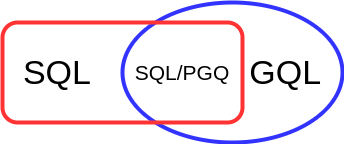
\includegraphics[width=0.5\linewidth]{figures/SQLPGQ-GQL.png}
  \caption{SQL/PGQ in relation to SQL and GQL.}
  \label{fig:sqlpgqgql}
\end{figure}

% Additionally, the standardised query language used in RDBMSs, SQL, will be releasing an extension called SQL/Property Graph Query (SQL/PGQ) in September 2022~\cite{Deutsch2021}. 
% This extension will make it easier to write queries with \textit{graph patterns} and navigational expressions in SQL.

In this thesis we integrate the SQL/PGQ standard in DuckDB.
DuckDB is an open-source in-process SQL OLAP database management system produced~\cite{DBLP:conf/sigmod/RaasveldtM19} by CWI~\cite{duckdblabs}. 
With the new SQL/PGQ standard releasing soon, work on integrating it into DuckDB has already started by Singh et al.~\cite{sqlpgq-duckdb}. 
However, the standard has not been fully integrated as of now. In particular the shortest and cheapest path functions are not yet implemented. Additionally, the feature to return the nodes contained in these cheapest and shortest path functions will also be implemented.
Therefore, the goal is to complete this integration by adding these functionalities. Additionally, we will identify and implement various optimizations especially related to typical graph queries in DuckDB.
% In the current state SQL/PGQ queries can be parsed and the reachability of a node, given a source node, can be computed. 
% The next step is to compute the path length and eventually be able to retrieve the path. 
% Essentially being able to compute various numbers of graph traversal operations. 

The structure of this thesis proposal is as follows. Section~\ref{sec:background} discusses relevant background information regarding graphs and SQL/PGQ. In Section~\ref{sec:goals} we formulate the research questions and the goals of this thesis. Section~\ref{sec:method} describes how the research questions will be answered and evaluated and provides a research plan. We end with a conclusion in Section~\ref{sec:conclusion}.  






% \subsection{Why is it interesting and important?}

% \subsection{Why is it hard? (E.g., why do naive approaches fail?)}

% \subsection{Why hasn't it been solved before? (Or, what's wrong with previous proposed solutions? How does mine differ?)}
% \subsection{What are the key components of my approach and results? Also include any specific limitations.}














% Graph databases have seen an increase in popularity in the last few years. 
% Graphs provide an intuitive way of storing and visualizing data, an example of this is Wikidata which stores its data in the form of open-source knowledge graphs~\cite{10.1145/2629489}. This data is provided in the Resource Description Framework (RDF) format, which is a form of direct edge-labelled graphs. Another way of storing data is by using the property graph data model, which is a form of a mixed multigraph model. In these models both nodes and edges can have labels, as well as properties, a more detailed description will be provided in Section~\ref{sec:background}. 

% Working with property graph data models in SQL is possible, however cumbersome and graph-based queries can be difficult to write and understand~\cite{graindb}. 
% Only recently has there been a proposal for the SQL standard to be expanded upon with the addition of the Graph Query Language (GQL)~\cite{gqlproposal}. 
% Initiative was taken in 2018 with the GQL manifesto~\cite{gqlmanifesto} by A. Green. 
% At the time, many separate graph query languages existed. However, three languages were chosen as the inspiration for GQL, namely Cypher originally created by Neo4j and currently maintained by OpenCypher, Property Graph Query Language (PGQL) by Oracle and G-CORE, a research language from the Linked Database Benchmarking Council (LDBC). 
% The proposal for GQL was accepted by the JTC1-the committee in joint charge of information technology standard for the International Organization for Standardization (ISO), and International Electrotechnical Commission (IEC)~\cite{Deutsch2021} and as such, the SQL standard will be extended with SQL/Property Graph Query (SQL/PGQ). SQL/PGQ specifies how graph views should be defined over an SQL tabular schema, and running read-only queries against them.  

% The main topic of this thesis is to integrate the SQL/PGQ standard as defined in DuckDB. DuckDB is an open-source in-process SQL OLAP database managament system produced by DuckDB labs, a spin-off company at CWI~\cite{duckdblabs}. With the new SQL/PGQ standard recently having been approved, work on integrating it into DuckDB has already started by Singh et al.~\cite{sqlpgq-duckdb}. However, the standard has not been fully integrated as of now. In the current state SQL/PGQ queries can be parsed and the reachability of a node, given a source node, can be computed. The next step is to compute the path length, and eventually be able to retrieve the path. Essentially being able to compute various numbers of graph traversal operations. 

% In addition, the performance of DuckDB can be further optimized in certain cases. In particular, when a query is executed containing a join operation on the same table ($Table A \Join Table A$), two hash tables are built for each table. However, these hash tables are equal and therefore only a single one would suffice, reducing memory usage and saving time on building the hash table. This case occurs often when querying graph tables in RDBMSs, since the graphs are stored in two tables, the vertex table (containing a $node_id$) and the edge table (containing a $source_node_id$ and a $destination_source_id$). Whenever a query is performed on these tables, we join the vertex table twice on the edge table (once on the $source_node_id$ and once on the $destination_node_id$). 

% In spirit, this thesis contains similarities to the work performed by Jin et al.~\cite{graindb}. They created GRainDB, a system which extended DuckDB with graph modeling, querying, and visualization capabilities. However, they based their query language GRQL from TigerGraph's GSQL~\cite{tigergraph} and Oracle's PGQL~\cite{10.1145/2960414.2960421}. Thus, this thesis differs in that the goal will be to integrate the standardized SQL/PGQ. 

% The structure of this thesis proposal is as follows. Section~\ref{sec:background} will discuss relevant background information regarding graphs and SQL/PGQ. In Section~\ref{sec:goals} we formulate the research questions and the goals of this thesis proposal. Section~\ref{sec:method} will describe how the research questions will be answered and evaluated and provides a small concrete planning. We end with a conclusion in Section~\ref{sec:conclusion}.  

% \subsection{Why would SQL/PGQ be better}






% \section{Background}\label{sec:background}
\subsection{Property Graph Data Model}
Graphs can be used to model complex, connected data through the use of vertices and edges. 
The vertices, sometimes referred to as nodes, represent objects.
The edges, also referred to as relationships, represent the relations between objects. 
The simplest form of a graph is the \textit{simple directed graph model}~\cite{DBLP:journals/corr/abs-1910-09017}. 
In this model, the graph consists of a set of vertices, and a set of edges.
Each edge has a source vertex and a destination vertex. In the case of an undirected graph, both vertices within an edge act as the source and destination vertex. 
Graphs can either be weighted or unweighted. In weighted graphs, an edge between two vertices contains a weight. This weight can be different for every edge. In unweighted graphs, all edges are of equal weight. This is important when determining the shortest or cheapest path between two vertices in a graph. In the case of an unweighted graph, the shortest path will also be the cheapest path, since all weights are equal. For a weighted graph, this need not be the case. 
% A graph can also be weighted, where weights are assigned to the edges.

The simple graph model suffices in certain cases, such as computing the reachability of a vertex from all other vertices. 
However, it is not possible to store any information in either the vertices or edges. 
For this we introduce the \textit{Labelled Property Graph (LPG)} model, which is often used in graph databases~\cite{DBLP:journals/corr/abs-1910-09017}. 
The simple graph model is now enriched with the ability to assign labels to both vertices and edges. 
A label can for example be 'Person', or 'Knows'. 
Depending on the specific implementation of the graph database there can either be one or multiple labels assigned to a vertex or edge~\cite{DBLP:conf/sigmod/AnglesABBFGLPPS18}. 
In addition to labels, there can also be properties assigned to vertices and edges. 
They can contain more specific information to the vertex or edge than the label. 
For example, a property could be (Age, 23) or (Name, Dani\"el).
Examples of database systems that have based their data model on the LPG model are Neo4j~\cite{neo4jgraphbook}, TigerGraph~\cite{tigergraph}, and Oracle PGX~\cite{pgx}.
% Formally denoted, properties are modeled as key-value pairs $p = (\textit{key},value)$ where $key \in K$ and $value \in W$. 
% $K$ and $W$ are sets that contain all possible keys and values.


% Another form in which graph data can be modelled is the \textit{Resource Description Framework} (RDF). An RDF is based on \textit{Directed Edge-labelled Graphs}~\cite{10.1145/3447772} which contains a set of vertices and a set of directed labelled edges between nodes. The vertices represent entities and the edges represent binary relations between the entities. Database systems such as BlazeGraph~\cite{blazegraph} and Amazon Neptune~\cite{amazonneptune} have based their data model on the RDF model, this is also referred to as \textit{triple store}. Every triple is of the form (\textit{subject}, \textit{predicate}, \textit{object}). 

% Ways exist for data to be transformed between LPG and RDF~\cite{DBLP:journals/corr/abs-1910-09017}, thus it can depend on the application of the data which data model is chosen. 
% How the graph data is stored in database systems is also system dependent. 
% Examples are tuple stores, document stores, key-value stores, wide-column stores, RDBMS, or Object-Oriented DBMS. 


\subsection{SQL/PGQ}
SQL/PGQ limits itself to read-only graph queries and how to define graph views over a tabular schema~\cite{Deutsch2021}. 
The two most important graph querying functionalities are graph pattern matching and path finding as described by Angles et al.~\cite{DBLP:journals/csur/AnglesABHRV17}. 
These functionalities become more accessible with the addition of SQL/PGQ and queries involving these can be more easily expressed~\cite{graindb, oracle-sql-example}.

With SQL/PGQ, graphs are stored as a set of vertex tables and edge tables, where each row in a vertex/edge table represents a vertex/edge in the graph~\cite{gql-survey}.
A graph can be defined using the SQL statement~\cite{Neo4j2018} found in Listing~\ref{app:sqlpgqcreate}. 
\begin{lstlisting}[caption=Creating a graph in SQL/PGQ, label=app:sqlpgqcreate] 
CREATE PROPERTY GRAPH <name> [WITH SCHEMA <schema>] [FROM <subquery>]
\end{lstlisting}
For example, if we wish to create the graph of Figure~\ref{fig:graph-friend}, symbolizing a group of friends who all studied at some university, we would use the following query: 

\noindent\begin{minipage}{\linewidth}

\begin{lstlisting}[caption=Creating a friend network graph in SQL/PGQ, label=app:sqlpgqfriendnetwork] 
CREATE PROPERTY GRAPH friend_network 
VERTEX TABLES ( Person PROPERTIES ( name, dob ), 
                University PROPERTIES ( name ) )
EDGE TABLES (   knows SOURCE Person DESTINATION Person NO PROPERTIES, 
                studentOf SOURCE Person DESTINATION University NO PROPERTIES )
\end{lstlisting}
\end{minipage}

\begin{figure}
  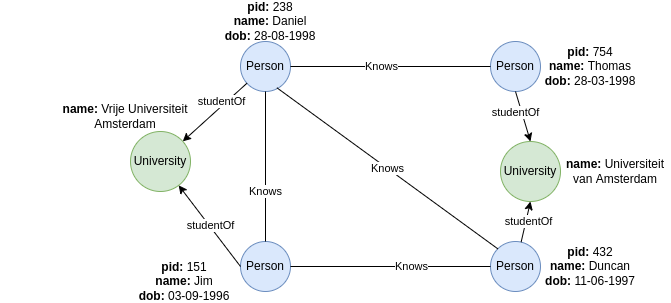
\includegraphics[width=\linewidth]{figures/friend-graph.png}
  \caption{Graph of friend network and where they study.}
  \label{fig:graph-friend}
\end{figure}


To match a pattern to this graph in SQL/PGQ, the \textcolor{blue}{\texttt{MATCH}} syntax can be used~\cite{Deutsch2021}, as can be seen in Listing~\ref{app:sqlpgqmatchnode}. 
% Matching graph patterns forms the core for many graph query languages and are sometimes also referred to as Regular Path Queries (RPQs)~\cite{Deutsch2021}.
For example, the following selects the name and date of birth from persons from the graph in Figure~\ref{fig:graph-friend} whose name is equal to 'Daniel': 
\begin{lstlisting}[caption=Pattern matching all nodes with the property name Daniel, label=app:sqlpgqmatchnode] 
SELECT p.name, p.dob
FROM Person GRAPH_TABLE (
    MATCH ( a:Person WHERE a.name = 'Daniel' )
    COLUMNS (
        a.name,
        a.dob )
    ) p
\end{lstlisting}

Matching such a simple graph pattern is also relatively straightforward in plain SQL, however, it could be argued that the SQL/PGQ syntax feels more natural to write than the plain SQL one, since it is closer to how the human mind tends to interpret the world regarding objects and their connections~\cite{benkler2008collective}. 
As can be seen in Listing~\ref{app:sqlpgqmatchnode}, we use the () notation to address a node. Addressing an edge can be done by using \texttt{[]}. To indicate that an edge is pointing from source to destination we use \texttt{(source)-[edge pattern]->(destination)}. This ASCII-art style is inspired by the syntax of Cypher, one of the most widely used graph query language~\cite{cypher-popularity}. 

A more complex graph pattern, involving both nodes and undirected edges could look like the following: 
\begin{lstlisting}[caption=Pattern matching using nodes and edges, label=app:sqlpgqmatchnodeedge] 
MATCH ( a:Person WHERE a.name = 'Daniel' )-[ e:knows ]-( b:Person )-[ f:studentOf ]-( c:University ) 
\end{lstlisting}

This statement would extract all patterns that match node $a$ being a Person with the name Daniel, who knows a Person who is a studentOf a University. Within every node or edge, we can filter the possibilities by adding a \textcolor{blue}{\texttt{WHERE}} statement, as can be seen in Listing~\ref{app:sqlpgqmatchnodeedge}.

One of the features of SQL/PGQ will be the ability to match a single edge pattern or a parenthesized path pattern for an arbitrary length~\cite{Deutsch2021}. 
An example where we want to find paths of length 2 to 5 of \textit{knows} edges: 
\begin{lstlisting}[caption=Path length of 2 to 5 knows edges, label=app:sqlpgqmatch25knows] 
MATCH ( a:Person )-[ e:knows ]->{2,5}( b:Person )
\end{lstlisting}
Finding such a path in plain SQL is significantly more difficult~\cite{oracle-sql-example}. 
SQL/PGQ is not limited to quantifying the upper-bound of the path length in such a path finding query. 
Similar to regular expressions, it is possible to use the Kleene star (*) operator, to indicate that the pattern can occur 0 or more times. 
Additionally, matching the pattern 1 or more times is possible using the Kleene plus (+) symbol.
The following is an example of a pattern using the Kleene star operator: 
\begin{lstlisting}[caption=Path length of arbitrarily many knows edges, label=app:sqlpgqmatchkleene] 
MATCH ( a:Person )-[ e:knows ]->*( b:Person )
\end{lstlisting}

Another addition in SQL/PGQ will be the ability to return the path corresponding to a query.
Alongside returning every path that adheres to a given pattern, it will be possible to return the cheapest or shortest path. 
The cheapest path will return the path in which the total weight of the edges along the path are the lowest.
The shortest path returns the path containing the least amount of hops from the starting node to the end node.
In case the graph is unweighted, cheapest and shortest path will provide equivalent results, since the weight of any edge will be equal to 1.
% A matching pattern containing the cheapest path will be of the format: 
% \begin{lstlisting}[caption=Matching the cheapest path, label=app:sqlpgqmatchcheapest] 
% MATCH CHEAPEST < pattern >
% \end{lstlisting}

% In the GQL manifesto~\cite{gqlmanifesto}, Green highlighted three similar query languages (Cypher, G-CORE, and PGQL) that coexisted, which he believed should be standardized into one. 
% Following will be a more in-depth look at those three languages, and how they differ from each other. 

% First, one of the most widely used query languages, Cypher~\cite{cypher-popularity} which was developed by Neo4j. 
% % It is currently an open-source project maintained by the openCypher Implementers Group~\cite{Francis2018}. 
% % One of the goals of providing an open-source language was to stimulate the transition from the openCypher implementation to the GQL standard and prevent a form of vendor lock-in~\cite{opencypher}. 
% A key feature of Cypher is the ASCII-art syntax for pattern matching. Additionally, if a vertex or edge with a specific label should be matched, one would write \texttt{(a:Account)-[r:Transfer]->{2..*}(b:Account)}. Here vertices (a) and (b) have the label 'Account', and the path is a directed edge as indicated by the arrow which has the label 'Transfer'.
% This intuitive syntax makes it an easy language to pick up~\cite{cypher-popularity}. 
% However, the query language has several shortcomings, namely the lack of regular path queries (RPQs) and graph construction~\cite{10.1145/2960414.2960421}. Regular path queries are recursive queries that define a path using regular expressions.

% The second graph query language is PGQL, which was created by Oracle Labs.
% PGQL follows a more SQL-like syntax and functionalities and provides functionalities for RPQs and graph construction.
% A PGQL query consists of three mandatory clauses \textit{SELECT}, \textit{FROM}, and \textit{WHERE} which can be followed by any of the optional clauses \textit{ORDER BY}, \textit{GROUP BY}, and \textit{LIMIT}. 
% The PGQL developers argue that the SQL-like syntax for PGQL allows existing SQL users to switch easily between the two languages~\cite{10.1145/2960414.2960421}. 

% The final graph query language from which inspiration was taken was G-CORE~\cite{DBLP:conf/sigmod/AnglesABBFGLPPS18}. The language was developed by the LDBC Graph Query Language Task Force~\cite{ldbc} which consists of members from industry and academia. The task force used the core of current existing graph languages as a base to develop G-CORE. They provide a formal definition of G-CORE to help correct the development of the language~\cite{gcoreparser}. The main deviation of G-CORE compared to other languages is how it treats paths as first-class citizens. It essentially means that paths become just as important as nodes and edges, allowing users to use paths in their queries. 

\subsection{Graph traversal algorithms}
\label{sec:graph-traversal}
\subsubsection{Multi-Source Breadth-First Search (MS-BFS)}
In order to compute the shortest path of unweighted graphs, the batched variant of the MS-BFS algorithm developed by Then et al.~\cite{10.14778/2735496.2735507} can be used. The pseudo-code of the algorithm is provided in Algorithm~\ref{alg:msbfs}. 
The algorithm is an example of a bulk algorithm that fits well in the vectorized execution engine of DuckDB~\cite{keynote-boncz-edbt-icdt-2022}. 
It is able to run multiple BFSs concurrently on the same graph in a single CPU core. 
Furthermore, it can make use of Single Instruction Multiple Data (SIMD) instructions, such as AVX-512~\cite{avx512}, that are available in modern CPUs. 
This lets us handle 512 BFS steps in one CPU cycle, further increasing the efficiency in CPU usage. 
Additionally, it has the ability to scale up as the number of CPU cores increases. Since there are no dependencies between the various BFSs, they can be divided over multiple cores. 
It makes use of the small-world property~\cite{smallworld} that occurs when the diameter of a graph is small in comparison to the total number of nodes.
This means that each BFS discovers most vertices in a few iterations, and concurrent BFSs have a high chance of overlapping sets of discovered edges in the same iteration. 
This allows access to be shared among the multiple BFSs and reduce the chance of cache misses, reducing the overall computation time~\cite{10.14778/2735496.2735507}.


\begin{algorithm}
\caption{MS-BFS}
\label{alg:msbfs}
\begin{algorithmic}[2]
    \State \textbf{Input:} $G,\mathbbm{B},s$
    \State $seen_{s_i} \leftarrow \{b_i\} \:for \: all \: b_i \in \mathbbm{B}$
    \State $visit \leftarrow \bigcup_{b_i \in \mathbbm{B}}\{(s_i,\{b_i\})\}$
    \State $visitNext \leftarrow \varnothing$
    
    \While {$visit \neq \varnothing$}
        \For {\textbf{each} $v \: \textbf{in} \: visit$}
            \State $\mathbbm{B}'_v \leftarrow \varnothing$
            \For {\textbf{each} $(v', \mathbbm{B}') \in visit \: \textbf{where} \: v' = v$}
                \State $\mathbbm{B}'_v \leftarrow \mathbbm{B}'_v \cup \mathbbm{B}'$
            \EndFor
            \For {\textbf{each} $n \in neighbours_v$}
                \State $\mathbbm{D} \leftarrow \mathbbm{B}'_v \setminus seen_n$
                \If {$\mathbbm{D} \neq \varnothing$}
                    \State $visitNext \leftarrow visitNext \cup \{(n,\mathbbm{D})\}$
                    \State $seen_n \leftarrow seen_n \cup \mathbbm{D}$
                    \State Do BFS computation on $n$
                \EndIf
            \EndFor
        \EndFor
        \State $visit \leftarrow visitNext$
        \State $visitNext \leftarrow \varnothing$
    \EndWhile   
\end{algorithmic}
\end{algorithm}


\subsubsection{Cheapest path}
To find a cheapest path in weighted graphs either the Dijkstra or Bellman-Ford algorithms can be used. The Dijkstra algorithm has a worst-case time complexity of $\mathcal{O}(|E|+|V|\log|V|)$~\cite{10.1145/28869.28874}, which is better than Bellman-Ford's worst-case time complexity of $\mathcal{O}(|V|\cdot|E|)$~\cite{bannister2011randomized}.
However, the expected runtime of Bellman-Ford is $O(|E|)$ in large dense graphs with low diameter~\cite{Yen1970AnAF}.
Then et al.~\cite{DBLP:journals/dbsk/ThenGKN17} propose a Batched Bellman-Ford-based algorithm, shown in Algorithm~\ref{alg:batched-bellman-ford}, to find the shortest distance between two nodes in a graph.
This algorithm can make use of SIMD instructions to increase the CPU usage efficiency, which is not possible with the standard Bellman-Ford algorithm~\cite{bellman1958routing}, which is shown in Algorithm~\ref{alg:bellman-ford}. 

\begin{algorithm}
\caption{Bellman-Ford}
\label{alg:bellman-ford}
\begin{algorithmic}[2]
    \State Initialize-Single-Source(G,s)
    \For {$i \leftarrow 1$ to $|V[G]| - 1$}
        \For {\textbf{each} edge $(u,v) \in E[G]$}
            \State Relax(u, v, w)
        \EndFor
    \EndFor
    \For {\textbf{each} $edge (u,v) \in E[G]$}
        \If {$d[v] > d[u] + w(u, v)$}
            \State Return False
        \EndIf
    \EndFor
    
 
\end{algorithmic}
\end{algorithm}

\begin{algorithm}
\caption{Directed batched Bellman-Ford-based algorithm}
\label{alg:batched-bellman-ford}
\begin{algorithmic}[2]
    \State \textbf{Input: WeightedGraph G, Array<Vertex>} sources
    \State \textbf{Output: VertexProperty<BatchVar<double>\>>} dists
    
    \State \textbf{VertexProperty<BatchVar<bool>\>>} modified = false
    \State dists = Infinite
    
    \For {i=1..sources.length}
        \State \textbf{Node} v = sources[i]
        \State dists[v][i] = 0
        \State modified[v][i] = true
    \EndFor
    
    \State \textbf{bool} changed = true
    \While{changed}
        \State changed = false
        \For{\textbf{each} v in G.vertices}
            \If{not modified[v].empty()}
                \For{\textbf{each} v in G.neighbours(v)}
                    \State double weight = edgeWeight(v,n)
                    \For{\textbf{each} i in modified[v]}
                        \State \textbf{double} newDist = min(dists[n][i], dists[v][i] + weight)
                        \If {newDist != dists[n][i]}
                            \State dists[n][i] = newDist
                            \State modified[n][i] = true
                            \State changed = true
                        \EndIf
                    \EndFor
                \EndFor
            \EndIf
        \EndFor
    \EndWhile
    
 
\end{algorithmic}
\end{algorithm}


\subsection{DuckDB}
DuckDB is a database management system specialized in OLAP workloads~\cite{DBLP:conf/sigmod/RaasveldtM19}.
This means that the system is optimized more towards analytical queries, touching large data volumes using joins and aggregations.
Just like SQLite, DuckDB is an in-process system, though SQLite is specialized in OLTP workloads.

DuckDB consists of a number of components: Parser, logical planner, optimizer, physical planner, and execution engine. 
The system can be accessed through a C/C++ API, as well as a SQLite compatibility layer. 
The SQL parser is based on the PostgreSQL SQL parser~\cite{DBLP:conf/sigmod/RaasveldtM19}.
The logical planner consists of a binder and a plan generator.
The binder is responsible for the expressions from the query related to anything containing a schema such as tables and views and retrieves the required columns and data types. 
The plan generator then creates a tree of basic logical query operators from the retrieved parse tree. 
Once the logical planner is done, the optimizer is used to optimize the logical plan. 
This will result in an optimized logical plan which is given to the physical planner where it is turned into a physical plan.
The physical plan consists of operators, where each operator implements one step of the plan. 
An example of a unary operator is the \textit{scan}, which scans a table and brings each tuple of a relation into main memory~\cite{DBLP:books/daglib/0020812}.
A join operator that makes use of two tables is an example of a binary operator.

These operators are split up into pipelines, which determines the order of operation execution.
A query can consist of one or more pipelines, some of which contain a dependency on another pipeline. 
A pipeline with a dependency is for example, one containing a \textit{join} operator. 
The start of a pipeline is referred to as a source and the end is referred to as the sink, which is where all the data is collected (materialized).
Only sink operators, such as sorting, building a hash table, and hash aggregation need to see all the data before they can proceed. All other operators do not need to materialize all data before proceeding. 
In the case of binary operators there are always two pipelines, one that builds the hash table, and one that probes this hash table. Both pipelines contain a source and a sink, and since the probing is a non-materializing operation it can be scheduled in the middle of a pipeline. 

With every join, a hash table needs to be built on which the join can be performed and the operator needs to wait for the entire hash table to be built.  
Only then can the join be correctly executed.
In the same vein, another pipeline might require the outcome of this join before it can be executed, creating a chain of dependencies.

DuckDB makes use of hash tables to perform join operations\footnote{Whenever the ids of the smaller table are dense, meaning the maximum id is not much larger than the size of the table, an array is used instead, eliminating the need to build a hash table. This is referred to as a perfect join~\cite{DBLP:conf/sigmod/AbadiMH08}.}. 
Cardinality estimation is performed to asses which of the two tables is the smaller one. These estimations can be wrong, so it is not guaranteed that the smallest table is always used. 



This smallest table is then used to build a hash table from, this is also referred to as the \textit{sink} or the build side. 
The other, larger, table is then used to probe the hash table, looking for matching entries, this is referred to as the \textit{source} or the probe side.
Whenever the two tables are of equal size, a random one of the two is chosen to be the sink. 

% After finalizing the physical plan, a pipeline is constructed in which the order of operator execution is determined.


The execution engine of DuckDB is vectorized~\cite{DBLP:conf/sigmod/RaasveldtM19}. The use of vectors is more CPU efficient than the more common tuple-at-a-time execution found in other DBMSs~\cite{DBLP:conf/cidr/BonczZN05}. 
ACID-compliance (\textbf{A}tomic, \textbf{C}onsistent, \textbf{I}solated, and \textbf{D}urable) in DuckDB is provided by Multi-Version Concurrency Control~\cite{DBLP:conf/sigmod/RaasveldtM19}.
To allow for persistent storage, DuckDB uses the DataBlocks storage layout, which is read-optimized~\cite{DBLP:conf/sigmod/RaasveldtM19}.
A useful feature of DuckDB is the allowance of extension modules, also referred to as Scalar user-defined functions (UDFs).
These Scalar UDFs are as fast as the built-in functions of DuckDB due to the vectorized query processing, meaning that the parallelization of the UDF is handled by DuckDB. 


\subsection{Current state of SQL/PGQ in DuckDB}\label{sec:sofar}
This thesis will make use of the work done by Singh et al.~\cite{sqlpgq-duckdb}. 
They identified several challenges that needed to be addressed. 
DuckDB is primarily intended for tabular workloads and wants to limit its core features to those required for the tabular types of workloads.
Therefore, minimal changes to the parser and transformer were made to allow correct parsing of SQL/PGQ queries.  
One of the first challenges to be tackled was successfully parsing SQL/PGQ queries. 
Modifications were made to the DuckDB parser to allow for the ASCII-art style query syntax that is introduced with SQL/PGQ as shown in Listing~\ref{app:sqlpgqmatchnodeedge}. 
Additionally, new statements like GRAPH, LABEL, PROPERTIES were added to the parser to allow for correct parsing of SQL/PGQ queries.
The SQL/PGQ queries are transformed into plain SQL queries using Scalar UDFs, an example of which can be seen in Listing~\ref{app:sqlpgqquery2} and Listing~\ref{app:sqlpgqquerykleene}. 

Some queries are more difficult to translate from SQL/PGQ to plain SQL. 
For instance, queries containing the Kleene star operator, shown in Listing~\ref{app:sqlpgqmatchkleene} are challenging to translate as discussed by Michels and Witkowski~\cite{oracle-sql-example}. The translation requires to make use of the recursive \textit{WITH} statement.
The translation for queries containing the Kleene star operator is not always correct at the time of writing. 
Therefore, one of the tasks for this thesis is to improve this translation and ensure its correctness. 

Another consequence of limiting the core features was the decision to implement the new operators, such as the batched MS-BFS algorithm~\cite{10.14778/2735496.2735507} described in Section~\ref{sec:graph-traversal}, as Scalar UDFs. 
With MS-BFS it is possible to compute the reachability of any number of nodes given one or more source nodes. 
DuckDB handles the parallelization for Scalar UDFs using the morsel-driven method~\cite{duckdb-morsel-driven}, which helps when scaling the batched MS-BFS algorithm.
Another benefit of implementing these operators as Scalar UDFs instead of expressions is the fact that little to no changes have to be made to the internals of DuckDB. 
To implement reachability, no further changes needed to be made to the parser and no new logical and physical operators had to be introduced. 

Another challenge Singh et al. looked at was the access patterns. 
Typically, a pointer-based data structure can be used for $O(1)$ lookup. 
In this case, every node contains a mini-index to all nearby nodes~\cite{indexfreeadjacency}. 
However, this becomes inefficient in the case of multiple traversals due to poor memory locality. 
An alternative is to make use of a Compressed Sparse Row (CSR) data structure.
With this data structure, the rowids of both the vertex and edge tables are condensed into integers in the range  $[0, |V|)$ and $[0, |E|)$.  
Most important are the edge tables, which are usually much larger, leading to a higher chance of poor memory locality. 
Thus, a Scalar UDF was introduced to create the CSR data structures. The CSR structure needs to be created for both the vertex and the edge table in order for the reachability function to work.   

A weighted directed graph is represented in Figure~\ref{fig:unweightedgraph}.
Vertices that share an edge contain a weight, ranging between $[0, 1)$ in this example. 
For example, the edge from vertex 1 to vertex 2 has a weight of $0.3$.
Figure~\ref{fig:csrunweightedgraph} shows the CSR representation for the graph in Figure~\ref{fig:unweightedgraph}. 
The \textit{Vertex array} contains offsets for the \textit{Edge array}. The Edge array holds the indices of destination vertices. To find all outgoing edges from a given source vertex, we take its index. The offset at the index of the Vertex array gives us the offset for the first outgoing edge in the Edge array and subsequently the index of the destination vertex. 
% destination indices for which there is an edge going from the source index to the destination index. 
For example, in Figure~\ref{fig:unweightedgraph} we observe the first edge from vertex 1 directs to vertex 2. 
For vertex 4, the first edge direct to vertex 1, therefore, the offset of the Vertex array at index 4 points to 1 in the Edge array. 
The offset between two Vertex array offsets can be used to determine the number of edges for a source vertex.
This condenses the matrix-like data structure into regular arrays, improving the memory locality. 
Additionally, the structure only needs to be created once, after which it is kept in memory. 
The work by Singh et al. only supports unweighted graphs. Thus, one of the goals is to extend the CSR structure by also supporting weighted graphs.

\begin{figure}
  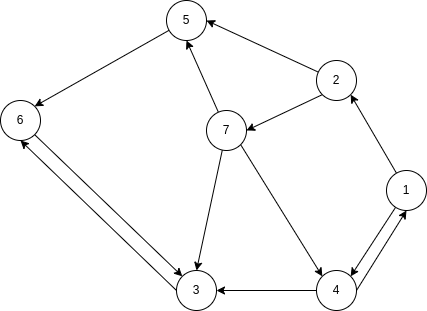
\includegraphics[width=0.6\linewidth]{figures/Graph-Unweighted-csr.drawio.png}
  \caption{An example of an unweighted graph}
  \label{fig:unweightedgraph}
\end{figure}


\begin{figure}
  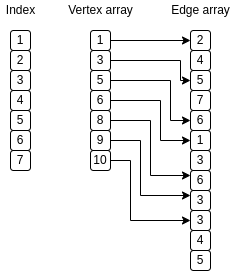
\includegraphics[width=0.6\linewidth]{figures/Unweighted CSR.drawio.png}
  \caption{CSR representation of the graph in Figure~\ref{fig:unweightedgraph}}
  \label{fig:csrunweightedgraph}
\end{figure}



\subsection{LDBC Social Network Benchmark}
The Linked Data Benchmark Council (LDBC) has created the Social Network Benchmark to test various functionalities of graph-like database management systems~\cite{DBLP:journals/corr/abs-2001-02299}. 
The benchmark contains datasets structured similarly to real-world social networks. 
Two workloads are described in the benchmark, the Interactive workload which focuses on interactive transactional queries, and the Business Intelligence workload that focuses on analytical queries. 
The latter is more relevant to this thesis as DuckDB is specialized towards analytical (OLAP) workloads~\cite{DBLP:conf/sigmod/RaasveldtM19}, thus making the workload better suited.

The Business Intelligence workload consists of complex read queries and refresh operations (insert and delete operations). Since SQL/PGQ is a read-only query language, we will only be focussing on the queries related to the read operations, of which there are 20. Each query contains a number of parameters which are generated before executing the query. These parameters are then used in the query to validate the correctness of the results. Various scale factors (SF) exist to help evaluate the scalability of the system.    

Three queries require to find a shortest or cheapest path from some starting point to a target. These queries are 15~\cite{snb-bi-15}, 19~\cite{snb-bi-19}, and 20~\cite{snb-bi-20}. 
Read query 20~\cite{snb-bi-20} provides two parameters: \texttt{Person2} and \texttt{Company}. 
The goal is to find \texttt{Person1} working or has worked at \texttt{Compay}, who has a connection with \texttt{Person2}. 
\texttt{Person2} is not working or has not worked at \texttt{Company}. 
This connection is defined by persons who know each other and have studied at the same university. 
The weight of the connection is an integer of the absolute difference between the year of enrolment + 1 (as to avoid division by zero errors).
Since the weights between any two persons are not all equal, it is necessary to calculate the cheapest path using the Batched Bellman-Ford algorithm discussed in Section~\ref{sec:graph-traversal}. In case all weights were equal, MS-BFS, also discussed in Section~\ref{sec:graph-traversal} could be used. 

For read query 19~\cite{snb-bi-19} the parameters are \texttt{City1} and \texttt{City2}. The goal is to find \texttt{Person1} and \texttt{Person2}, who are from their respective city, where the interaction path is the cheapest. The interaction path is defined as the number direct reply \texttt{Comments} to a \texttt{Message} by the other \texttt{Person}. More interactions imply a cheaper path, calculated by $1 / \textrm{count(interactions)}$, resulting in a 32-bit float. This means that the implementation of the cheapest path should work with both integers and floating point numbers. 

Query 15~\cite{snb-bi-15} involves a number of steps. At the start, two \texttt{Persons} are given as parameters. For these, the weighted shortest path needs to be calculated using the \texttt{knows} relation. The weight for any \texttt{knows} edge is calculated based on the interactions between the source and destination persons. Every direct reply from one person to a \texttt{Post} of the other person adds 1.0 interaction point. Every direct reply to a comment from one person to a \texttt{Comment} by the other person adds 0.5 interaction point. Only messages that are within a given \texttt{[startDate, endDate]} are considered. The edges are undirected, thus the interaction score is equal in both directions. The overall weight is calculated by $1 / (\textrm{interaction score} + 1)$

Furthermore, we will be making use of query 13 of the interactive workload. This query can be used to evaluate the performance of the shortest path algorithm. For this query we are given two parameters \texttt{Person1} and \texttt{Person2}, for which we have to find a shortest path through the \texttt{knows} table. If a path can be found, we should return the length of the path. If no path is found, we should return -1 as the distance. It can be the case that \texttt{Person1} is the same as \texttt{Person2}, in that case we should return 0. The complexity in this query is the search space that is given. Unlike with the queries discussed from the BI workload, we cannot perform a filter on the number of edges in the graph. In this case, we have to potentially consider all \texttt{knows} edges that are provided in the dataset. 


% \section{Methodology}\label{sec:method}
\subsection{Shortest path}
Computing the shortest path between two vertices in an unweighted graph can be done using MS-BFS. 
In the current implementation by Singh et al., it is possible to determine the reachability of a node. 
However, to determine the shortest path, some form of state needs to be kept, such that it can be tracked how many hops have been done before reaching the destination node. 
Often, graphs have the small-world property, the distance between any two nodes is very small compared to the size of the graph~\cite{10.14778/2735496.2735507}. 
In addition, the shortest distance is always smaller than or equal to the diameter, the greatest distance between any two nodes, of the graph.
Therefore, in unweighted graphs, the size of the values needed to be stored in memory can also be relatively small. 
For every source node for which the shortest distance is computed, it will likely be enough to store the distance within 8 bits. 
Since the distance can never be negative, an unsigned 8-bit integer would suffice, in the case that the diameter of the graph is less than 255. 
However, we should care not to exceed this limit as the integer will overflow, causing it to wrap around to 0. 
Whenever that would happen we should copy the values into 16-bit or 32-bit unsigned integers to ensure no overflow errors occur.
This does reduce the efficiency of the MS-BFS algorithm compared to the reachability implementation. 
Computing the reachability only requires a 1-bit bool value per BFS, which is set to 1 in case the destination node is reachable, 0 otherwise. 
Using the AVX-512 operation, it is possible to execute 512 reachability searches at once. 
However, since computing the shortest path requires at least 8 bits to keep track of the distance, it will only be possible to execute $512/8 = 64$ BFS searches at a time. 
If we were to use 32-bit integers, only 16 BFS searches could be run.
Unsigned integers are preferred over signed, since the length of a path can never be negative, there is no need for negative integers. Denoting that a node is unreachable can be done by using \texttt{UINT\_MAX}~\cite{uint-max}. During execution, we keep track of the depth of the MS-BFS. Whenever this depth reaches \texttt{UINT\_MAX}, we know there is a chance for an overflow and make sure this is handled correctly.

To compute the cheapest path in weighted graphs, there are typically two algorithms that can be used, Dijkstra's algorithm using a Fibonacci heap and the Bellman-Ford algorithm.
% The Bellman-Ford algorithm has a worst-case time complexity of $O(|V|*|E|)$, however the expected runtime for large dense graphs is $O(E)$~\cite{DBLP:journals/dbsk/ThenGKN17}.
Then et al.~\cite{DBLP:journals/dbsk/ThenGKN17} propose a batched Bellman-Ford algorithm to compute the geodesic distance in weighted graphs. 
They find that the performance of the Bellman-Ford algorithm is 3-10x higher compared to a batched variant of Dijkstra's algorithm~\cite{DBLP:journals/dbsk/ThenGKN17}.
Therefore, we will first look to implement the batched Bellman-Ford algorithm proposed by Then et al. as shown in Algorithm~\ref{alg:batched-bellman-ford}. 
Implementing a batched version of Dijkstra's algorithm will be more complex.
During the batched version multiple instances of Dijkstra's algorithm will run, each having its Fibonacci heap.
Given that each heap will be of a different structure, the effectiveness of possible SIMD instructions will be reduced. 
Therefore, it is not likely that a batched version of Dijkstra's algorithm will outperform the batched version of the Bellman-Ford algorithm. 
To test the performance of the implementations we will be using the LDBC Graphalytics benchmark~\cite{DBLP:journals/pvldb/IosupHNHPMCCSAT16}, which is designed to test various algorithms such as single-source shortest path (SSSP) and BFS.
Additionally, we will be using the LDBC Social Network Benchmark~\cite{DBLP:journals/corr/abs-2001-02299} to further test the performance of the implementations.


\subsection{Shared hash join}
Queries can contain multiple expensive joins which are in essence identical. This also happens in graph-like queries, where it is common to join the vertex table twice on the edge table. Once for the source of the edge, and once for the destination of the edge. 

In the current state of DuckDB, for each join a hash table is built from the smaller table. 
However, this is wasteful in the case where queries containing multiple join operations have identical sinks. 
For example, there exists a vertex table \textit{Person} containing the column \texttt{person\_id}, and an edge table \textit{Knows} containing the columns \texttt{person1\_id} and \texttt{person2\_id}. These tables are used to build a CSR representation for the edge table. 
Thus, it is necessary to perform two joins, namely $\texttt{person1\_id} \Join \texttt{person\_id}$ and $\texttt{person2\_id} \Join \texttt{person\_id}$. 
In this case, the right side is identical in both joins. 
See Figure~\ref{fig:physicalplanhashjoin} for the relevant part of the physical plan of this example query.
An optimization is to build this hash table only once, and reuse it for any identical joins containing the same sink. 
This will eliminate the need to build the same hash table multiple times.

\begin{figure}
  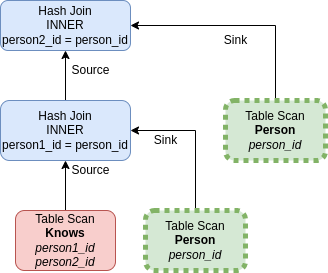
\includegraphics[width=0.6\linewidth]{figures/physicalplan-shared-hash-join.png}
  \caption{Example of a duplicate sink state in the physical plan}
  \label{fig:physicalplanhashjoin}
\end{figure}

The plan for the shared join optimization is to make the sink shareable between multiple pipelines in the case where the joins are identical. 
This will eliminate the need of building multiple identical hash tables since they can be reused. 
During the building phase of the pipelines, we will save all join operations we come across in combination with its respective pipeline. 
In the case where a duplicate join is encountered will the sink state of that pipeline be shared with the sink state of the pipeline seen earlier. 
In addition, the dependency of the parent pipeline on the current pipeline needs to be changed.
The optimization can not be performed on FULL or RIGHT joins. 
For these joins a state needs to be kept for the hash tables to see if a particular value has been accessed or not.
This access may vary between joins, and thus will result in different states. 
Therefore, the hash table cannot be reused for these types of joins. 

% Additionally, a case where the two joins make use of the same table but with different columns has to be taken care of.
% A solution would be to use the union of these columns to build the hash table. 



% A similar optimization can be performed for identical table scans. 
% Table scans are unique to a pipeline, and thus it is not known for other pipelines which tables have been scanned. 
% An optimization is to share table scans in case multiple identical ones are encountered in the query, removing the need for multiple table scans.

% A case needing to be considered with both joins and table scans is when 


% In DuckDB, an optimization rule will be added called 'Shared Hash Join'. During the optimization phase, the rule will be used to identify all tables used in combination with a join statement and store the table name in the client context of the query. 
% It is not sufficient to store the alias of the table (In Listing~\ref{lst:duplicatejoin} p, p2, and k), since these are likely different even if the same table is used.
% Storing only the table name can work initially, though more information is needed, such as possible filters applied on any of the joins.

% During the logical planning stage, a tree of basic logical query operators is built. 
% Examples of these are \textit{get} or \textit{comparison join} operators. 
% The get operator has no children, since this is the instruction to retrieve a specific table. 
% A comparison join operator has two children, the two operators which will be joined at a later stage. 

% \begin{figure}
%   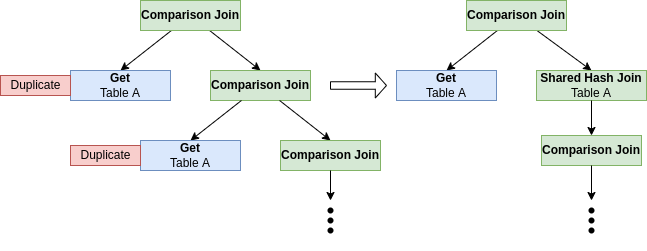
\includegraphics[width=0.75\linewidth]{MSc-thesis/figures/Sharedhashjoinlogicalplanner.png}
%   \caption{Logical query operator tree optimization}
%   \label{fig:sqlpgqgql}
% \end{figure}

% During the optimization phase, we will identify the tables on which joins are performed. 
% If we identify a join on a table that is seen previously, i.e. an identical join, we will swap the comparison join operator for a shared hash join operator. 
% Once the tree has been traversed, all duplicate joins will have been identified and been replaced by the shared hash join. 

% After the optimization, a physical plan is created from the resulting query tree.
% Within this plan, every join has a unique state containing among other things the hash table. 
% For the shared hash join, this state has to be shared between multiple join operations. 
% In addition, other operations could be dependent on the outcome of the join operation. 
% When using the shared hash join, we should correctly identify the dependencies of the join operator and link these to the shared hash join operator instead.



% This is important since it is not possible to use a copy of a hash table that is yet to be built.
% Within the physical planner, it should be checked whether the hash table for a given table has been built. 
% If it is, we do not build a new hash table, instead, we point to the already build hash table. 
% If it is not yet built, we will proceed as normal and build the hash table. 

% A possible edge case is when the joins are very similar, but each retrieve different columns. 
% In this case, the union of columns should be taken such that both tables have all columns required for the query. 
% Another case is when a filter is applied on one of the joins, but not on the other, otherwise identical, joins.

% In some cases, the various joins make use of hash tables with identical contents. 
% In this case, it is wasteful to build these duplicate hash tables more than once. 
% Instead, it is better to build the hash table once, and allow it to be reused by the other joins. 
% A specific example where this is the case is during the building of the CSR-like data structure for SQL/PGQ queries, as described by Singh et al.~\cite{sqlpgq-duckdb}.

%  However, in the case of Listing~\ref{lst:duplicatejoin}, the multiple joins will result in multiple identical hash tables for the smaller of the two tables in the join. 
% The optimization identified is to only build the hash table once, and allow it to be reused when duplicate joins are found.


In DuckDB, unit tests can be written using the \textit{SQLLogicTests framework} to test the correctness of the implementation~\cite{duckdb-testing}. 
Assuming that the implementation works correctly, we will be testing the performance of the optimization using the CSR creation queries used by Singh et al.~\cite{sqlpgq-duckdb}. These queries contain a duplicate join on the vertex table.
% Additionally, of the TPC-H benchmark, query 21 (see Listing~\ref{lst:tpc-h-query21}) contains a duplicate join that can be used to test the performance. 
By performing tests with and without the optimization, we should see that the queries using the optimization have a lower run-time. 

% \begin{lstlisting}[caption=TPC-H Query 21, label=lst:tpc-h-query21] 
% -- TPC-H Query 21

% SELECT
%     s_name,
%     count(*) as numwait
% FROM
%     supplier,
%     lineitem l1,
%     orders,
%     nation
% WHERE
%     s_suppkey = l1.l_suppkey
%     AND o_orderkey = l1.l_orderkey
%     AND o_orderstatus = 'F'
%     AND l1.l_receiptdate > l1.l_commitdate
%     AND EXISTS (
%         SELECT *
%         FROM lineitem l2
%         WHERE
%             l2.l_orderkey = l1.l_orderkey
%             AND l2.l_suppkey <> l1.l_suppkey
%     )
%     AND NOT EXISTS (
%         SELECT *
%         FROM lineitem l3
%         WHERE
%             l3.l_orderkey = l1.l_orderkey
%             AND l3.l_suppkey <> l1.l_suppkey
%             AND l3.l_receiptdate > l3.l_commitdate
%     )
%     AND s_nationkey = n_nationkey
%     AND n_name = 'SAUDI ARABIA'
% GROUP BY
%     s_name
% ORDER BY
%     numwait desc,
%     s_name
% LIMIT 100
% \end{lstlisting}






% This section will provide details on how the research topics will be tackled and evaluated. A small planning is also provided. 

% \subsection{How will the problems be tackled}
% Work on integrating SQL/PGQ into DuckDB is currently being done in a publicly available GitHub repository~\cite{sqlpgqduckdbrepo}. Any further work done on integrating SQL/PGQ in DuckDB will be performed in this repository. In the current implementation, reachability has been implemented as a User Defined Function (UDF) in DuckDB. Creating UDFs will likely be the optimal way of implementing functions with which the path length and the actual path can be retrieved. 
% Once the UDFs have been implemented they should be benchmarked using the LDBC Graphalytics Benchmark~\cite{DBLP:journals/corr/abs-2011-15028}. This open-source industrial-grade benchmark consists of several deterministic algorithms for graph analysis and provides a fair comparison to other graph-based systems~\cite{DBLP:journals/corr/abs-2011-15028}. 

% Work on optimizing the hash tables will also be done in the same repository~\cite{sqlpgqduckdbrepo}. However, before the optimization can be implemented, it should be discussed with the development team of DuckDB to decide on the optimal way to implement it. Once implemented, the optimization should be faster consume less memory, as only one hash table needs to be built instead of 2 or more. The optimization can be compared to a version without the optimization to assess its effectiveness. Apart from the optimization, as much as possible between the two systems should be the same to provide a fair comparison.  

% To the best of our knowledge, currently, no standard test suite exists to analyse the performance of the SQL/PGQ integration in a relational database. Therefore, one of the goals of this thesis is to create such a test kit. The kit should involve a wide variety of graph patterns and navigational expression queries to provide a comprehensive test. These tests should then be benchmarked and compared to other GDBMSs such as Neo4j~\cite{Neo4j2018}, TigerGraph~\cite{tigergraph}, and GRainDB~\cite{graindb}.



% see Listing~\ref{lst:duplicatejoin} for example. This example contains a triangle query where the data of \textit{knows} and \textit{person} tables are joined multiple times on the same keys.
% \begin{lstlisting}[caption=SQL query containing identical joins, label=lst:duplicatejoin]
% SELECT p.pid, p2.pid 
% FROM person p, knows k, person p2, knows k2, person p3, knows k3 
% WHERE p.pid = k.pid 
%     AND p2.pid = k.kid 
%     AND p2.pid = k2.pid 
%     AND p3.pid = k2.kid 
%     AND p3.pid = k3.pid 
%     AND p.pid = k3.kid
% \end{lstlisting}


\subsection{Planning}
See Table \ref{tab:planning}.


\begin{table}[]
\begin{tabular}{|l|l|}
\hline
\textbf{Month} & \textbf{Goals}                                                                                                 \\ \hline
February       & \begin{tabular}[c]{@{}l@{}}Work on literature study \\ Start on optimization shared hash tables\end{tabular}   \\ \hline
March          & \begin{tabular}[c]{@{}l@{}}Work on optimization hash tables\\ Start on shortest path using MS-BFS\end{tabular} \\ \hline
April          & \begin{tabular}[c]{@{}l@{}}Finish optimization hash tables\\ Finish shortest path and experiment\end{tabular}  \\ \hline
May            & \begin{tabular}[c]{@{}l@{}}Start on cheapest path using \\batched Bellman-Ford / Dijkstra\end{tabular}         \\ \hline
June           & \begin{tabular}[c]{@{}l@{}}Finish cheapest path \\ Start on experimenting\end{tabular}                         \\ \hline
July           & \begin{tabular}[c]{@{}l@{}}Finish up experimenting\\ Finish up writing\end{tabular}                            \\ \hline
\end{tabular}
\caption{Initial planning
}
\label{tab:planning}
\end{table}





% \input{sections/discussion}
\section{Threats To Validity}\label{sec:threats}



\subsection{Internal Validity}
\subsection{External Validity}
\subsection{Construct Validity}
\subsection{Conclusion Validity}
\section{Related Work}\label{s:related}
\subsection{Scopus Query}
TITLE-ABS-KEY(DATABASE) AND ( TITLE-ABS-KEY("*GRAPH PATTERN MATCHING*") OR TITLE-ABS-KEY("*PATH FINDING*") OR TITLE-ABS-KEY("*GRAPH QUERY LANGUAGE*") ) AND ( LIMIT-TO ( PUBYEAR,2022) OR LIMIT-TO ( PUBYEAR,2021) OR LIMIT-TO ( PUBYEAR,2020) OR LIMIT-TO ( PUBYEAR,2019) OR LIMIT-TO ( PUBYEAR,2018) ) AND ( LIMIT-TO ( SUBJAREA,"COMP" ) ) AND ( LIMIT-TO ( LANGUAGE,"English" ) )

\subsection{Graph Pattern Matching in GQL and SQL/PGQ}

\url{https://arxiv.org/pdf/2112.06217.pdf} 
GQL and SQL/PGQ share a common graph pattern matching language (GPML) -> Extracts data from a graph which matches a graph pattern -> result is a set of path bindings where each variable is mapped to a node or edge in the graph. The main difference between GQL en SQL/PGQ is the way the data is represented, with the latter showing it in table form. 
A brief introduction of graphs is given. They consist of nodes which are connected with edges. Both can carry labels (Account, City, Transfer) and key/value pairs (isBlocked/No). Graphs can be either directed, partially directed or undirected. There can be multiple edges between two nodes. Self-loops are also possible. A path is an alternating sequence of nodes and edges, starting and ending with a node and subsequent nodes are connected with edges.
Several conjuctive regular path queries (CRPQs) exist, such as SPARQL, Cypher, Oracle PGQL and TigerGraph’s GSQL

A GPML pattern is as follows MATCH pattern optionally followed by a WHERE 
	MATCH (x:Account WHERE x.isBlocked = ‘No’)
	MATCH(x) -> x here is called a element variable (node patterns)
	MATCH -[e]-> -> e (edge patterns)

There are also quantifiers, similar to regex
{m,n} between m and n repetitions
{m, } m or more repetitions
* 0 or more repetitions
+ 1 or more repetitions. 

Two forms of union
path pattern union (using |)
multiset alternation (using |+|)
Conditional variables (Need to understand better)

To figure out the direction of an edge (What happens here with undirected edges, what is the the outcome of IS SOURCE OF and IS DESTINATION OF
e IS DIRECTED -> true if e is bound to a directed edge
s IS SOURCE OF e -> true if s is bound to the source of e
d IS DESTINATION OF e -> true if d is bound to the destination of e 

GPML queries must demonstrably terminate, this is done using restrictors and selectors. 
Restrictor: Path predicate (imposes a condition stating which paths are acceptable) such that the number of matches cannot be infinite) 
TRAIL no repeated edges
ACYCLIC no repeated nodes
SIMPLE no repeated nodes, except that the first and last nodes may be the same
Selector: Algorithm that conceptually partitions the solution space on the endpoints and selects a finite set of matches from each partition. 
ANY SHORTEST selects one path with shortest length from each partition
ALL SHORTEST selects all paths in partition that have minimal length
ANY selects one path in each partition arbitrarily
ANY  K selects arbitrary path ks in each partition
SHORTEST K select shortest k paths
SHORTEST K GROUP Groups with same length k, selects all paths in the first k groups. 

Key steps in pattern matching execution model 
Normalisation
Expansion 
Rigid-pattern matching
Reduction and deduplication

Graph database applications with SQL/PGQ
\url{https://download.oracle.com/otndocs/products/spatial/pdf/AnD2020/AD_Develop_Graph_Apps_SQL_PGQ.pdf}
Contains a good example on the use of graph view (Anti-Money Laundering)
Query is shorter and more intuitive

\subsection{Query, Analysis, and Benchmarking Techniques for Evolving Property Graphs of Software Systems by Gábor Szárnyas – PhD dissertation, BME (2019)}

Conceptual graph data models~\cite{Szrnyas2019QueryAA}
Untyped graphs: hold no type information
Definition 1 (untyped graph or homogeneous graph) G = (V,E,src,trg) where V is a set of nodes, E a set of edges. Functions src,trg : $E \rightarrow V$ are total functions respectively assigning the source and target node to each edge. 
Definition 2 (graph elements) We refer to the union of nodes and edges as graph elements
Definition 3 (weighted graphs) A weighted graph is a graph where each edge is assigned a weight $w \in \Re$
Definition 4 (edge-typed graph or multiplex graph) An edge-typed graph is defined as G = (V,E,src,trg,T,type), where T is a set of edge types and function type $E \rightarrow T$ assigns a single type to each edge. Useful since we still abstract away information regarding the node labels, but provides more insight compared to untyped graphs. 
Definition 5 (node-labelled graph) Defined as G = (V,E,src,trg,L,labels), where L is a set of node labels, and function labels : $V \rightarrow 2^L$ assigns a set of labels to each node
Definition 6 (labelled graph) G = (V,E,src,trg,L,T,labels,type)

Definition 7 (property graph) G = (V,E,src,trg,L,T,labels,type,Pv,Pe)
$P_v$: set of node properties. $p \in P_v$ is a function p : $V \rightarrow D$, which assigns a property value $d \in D$ to node $v \in V$, if v has property p, otherwise returns NULL    
$P_e$: set of edge properties. $p \in P_e$ is a function P : $E \rightarrow D$, which assigns a property value $d \in D$ to edge $e \in E$, if e has property p, otherwise returns NULL 

Path property graphs mentioned in G-CORE, treating paths as first-class citizens by introducing an explicit set of paths in the data model, each path having its own set of labels and properties.

Practical graph data models
Eclipse Modelling Framework (EMF) 
EClass represents classes. Identified by their name and may have several attributes and references. Can refer to supertype classes.
EAttribute represents attributes which contain data elements of a class (contain data type)
EDataType represents simple data types that are treated as atomic
EReference represents unidirectional edge between EClasses identified by their name. LowerBound and UpperBound can be specified

Property graphs are common in graph databases. No or optional support provided for metamodelling features. 

Semantic Graphs (RDF)
Provides metadata data model for semantic web applications. 
Makes a statement about resources (nodes/objects) in the form of triples. A triple is composed of a subject, a predicate and an object. Both ontology (metamodel) and facts (instance model) are represented as triples and stored together in the knowledge base. 
Specialised databases for triplestores
Semantic graphs can be modelled as labelled graphs. 

Relation model 
RDBMSs dominating
Database schema with attribute types and primary and foreign key relations and integrity constraints. 

Schema inference algorithm. Lack of predefined schema is so prevalent that an algorithm has been designed to work around this problem by extracting the relevant part of the schema from the query specifications. 

Nodes and edges are mapped to tuples
Nodes are represented by 1-tuples
Edges are represented by triple (source node, edge, target node)
Often useful to specify the attribute names for each tuple

Unary operators
Definition 8 (projection) $\pi$ filters the attributes (columns) of a relation by only keeping a certain set of them. Can also be extended to perform computations and produce new attributes. 
Definition 9 (selection) $\sigma$ filters the relation according to some criteria. $t = \sigma_\theta(r)$ where $\theta$ is a propositional formula. Selects all tuples in r for which holds. 
Definition 10 (duplicate elimination) $\delta$ eliminates duplicate tuples in a bag. 

Binary operators
Definition 11 (union) produces the set union of the tuples in the relations
Definition 12 (bag union) bag union of two relations produces the bag (multiset) union of the tuples in the relations (uniqueness not required). 
Definition 13 (set minus) On two relations, removes the tuples present in the second relation from the first relation. 
Definition 14 (Cartesian product) $t = r x s$, where t holds all tuples that are concatenations of exactly one tuple from r and exactly one tuple from s. 
\begin{equation}
	r \times s = {(r1,..., r_m, s1,..., s_n) | (r1,...,r_m) \in r \wedge (s1,...,s_n) \in s}
\end{equation}
Definition 15 (join or natural join) Producing the cartesian product of the relations, then filtering those tuples which are equal on the attributes that share a common name. When a tuple appears in both, we only keep a single one. 
Definition 16 (semijoin) takes its left input and only keeps tuples which have a matching pair on its right input in a join. 
Definition 17 (antijoin) Collects tuples from the left relation r which have no matching pair in the right relation s
Definition 18 (left outer join) Produces the join of its input relations, then adds tuples from the left relation that did not have a pair in the right relation and pads them with NULL values. 

Definition 19 (theta-joins) Performs the join according to a predicate $\theta$ a propositional formula

Definition 20 (theta-antijoin) 

Graph pattern matching against a graph instance is widely known as the graph isomorphism problem. 
Isomorphism-based semantics constrains some kinds of repetitions: 
No repeated node semantics → fully isomorphic matching and identical to restrictions used in the graph isomorphism problem
No repeated edge semantics is known as edge-isomorphic matching
Homomorphism based semantics defining no constraints on repetitions


Definition 21 (walk) sequence of nodes and edges, with both endpoints of an edge appearing adjacent to it in the sequence
Definition 22 (trail) a walk with no repetitions of edges
Definition 23 (path (strict) or simple path) a trail with no repetition of nodes. 
Definition 24 (path (relaxed)) same as walk
Definition 25 (shortest path) consists of a walk with the least amount of possible edges between two nodes 
	Can also be weighted if the edges contain weights
Definition 26 (distance) The length of a shortest path between two nodes
Definition 27 (cycle or circle) a walk that starts and ends in the same node

Graph queries: queries that contain graph patterns and / or path expressions. 
Recursive queries: queries that reference themselves and are evaluated up to reaching a fixpoint. 
Regular path queries (RPQs) are a restricted category of recursive queries that define paths using regular expressions. Allowing a concise formulation of graph queries, however little support so far. 
Path unwinding: allow users to define additional operations over a path in the graph

Support for WITH RECURSIVE was added in SQL:1999

Graph Query languages
Cypher
Supported by Neo4j. Making graph patterns with ascii-style 
Supports paths, transitive reachability or shortest paths. Supports path unwinding

PGQL 
Oracle labs
Combines SQL with graph pattern matching using Cypher-like syntax. 
Reachability and path finding queries are supported. 

G-CORE
Designed to meet two key goals 
Allow composition of queries → queries return graphs as their results
Treat paths as first class citizens → defined over the path property graph data model. 
Supports RPQs

SPARQL
For RDF 
Supports variants of RPQs with property paths allowing sequences, alternatives, inversions, and transitive edges. Only endpoints can be accessed. 

VIATRA Query Language
Defining graph patterns based on Datalog
Supports recursive queries in the form of recursive pattern calls. 


Two main categories of graph processing: 
Graph query workloads: typically run graph pattern matching and navigation operations on semantic or property graphs. Falls in different categories depending on the scope of the graph query
Local graph queries (For example on the neighbourhood of a node), more like OLTP style database systems
Global graph queries (OLAP) touch on a significant portion of the data, performing more complex aggregations on the data. 
Graph analysis workloads: define analytical computations on graphs with little to no information stored as attributes
Used to derive graph metrics, such as centrality, clustering and connectivity



\subsection{Cypher: An Evolving Query Language for Property Graphs}
Cyper property graph query language originally designed as part of Neo4j graph database~\cite{Francis2018}. 
Used in domains such as master data and knowledge management, recommendation engines, fraud detection, IT operations and network management, authorization and access control, bioinformatics, social networks, software system analysis and investigative journalism. 
Advantage of explicit support for graph data
In this paper Cypher 9 is discussed
Data model → property graphs, consisting of nodes and relationships (edges)
The language has a fully formalised semantics of its core constructs. Given the (at the time) lack of standard for the language, there was a need to provide this. 

Linear queries: Input is a property graph, output is a table. Instead of a SELECT statement at the beginning, there is a RETURN statement at the end of a query.
Queries can be merged together using a WITH statement, where the query before the WITH is the driving table for the query after the WITH. UNION is also supported. 

Pattern matching is done with ASCII art. Whatever binds to the pattern is introduced as a new row. The patterns express a restricted form of regular path queries: the concatenation and disjunction of single relationship types as well as variable length paths. 

Data can also be modified, using CREATE, DELETE and SET. A MERGE can also be performed using a pattern.
Overall the language is fairly similar to SQL, to allow users to switch easily between the two languages. 

Query execution follows a conventional model, outlined by Volcano Optimizer Generator. Query planning based on the IDP algorithm using a cost model. Final query compilation uses either a simple tuple-at-a-time-iterator-based execution model, or compiles the query to Java bytecode with a push-based execution model. 

Execution plan contains largely the same operators as RD engines, with an additional expand operator which finds pairs of nodes connected through an edge.

Several example queries are provided to create an understanding of the structure and execution of the queries. 

A formal specification is provided for the core of Cypher. 
Key elements: 
Data model, including values, graphs and tables
Query language, including expressions, patterns, clauses and queries
Values can be simple or composite, such as lists or maps. Expressions denote values, patterns occur in MATCH statements. Queries are sequences of clauses. Each clause denotes a function from tables to tables. 

A detailed description is provided of the values, the property graphs and tables. 
For paths of a set length, only one mapping exists of the free variables in which the path satisfies the pattern. In variable length paths this need not be the case. 
With rigid patterns, Cypher only looks in which relationship ids occur at most once. It cannot traverse the same relation more than once. Does not allow repeating relationship edges while matching patterns to avoid infinite paths. 

A detailed description on the semantics of clauses is provided

Limitation is that it does not support multiple graphs (disconnected) 
Named queries are supported in Cypher 10
Temporal types (like DateTime) are currently being developed
It is schema optional


\subsection{G-CORE A Core for Future Graph Query Languages}
G-CORE is a combined effort of academia and industry constructing the future of graph query languages~\cite{ctx13027080550005131}. Its main ideas are that the language should be composable, meaning that graphs are both the input and output of queries. Secondly, paths should be treated as first-class citizens. 
LDBC has designed G-CORE, as well as various graph data management benchmarks. 
Graph databases are useful in a wide variety of fields. 
Three main challenges are identified about existing graph query languages
Composability: Current implementations output tables of values, nodes or edges, while outputting graphs should make it easier for the user. 
Paths as first-class citizens: Providing the ability to return paths to the user enables post-processing paths within the query languages rather than in an ad-hoc manner
Capturing the core of available languages: Since no standard exists, current languages should be taken into account and what they do well in order to create a standard.
The following contributions are presented:
Path Property Graph Model: the property graph is extended with paths. Paths can also have labels and kv pairs. 
Syntax and semantics of G-CORE
Complexity results
Every query returns a graph. 
Complexity analysis: each query q over input PPG G can be computed in polynomial time. 
G-CORE and SQL can be combined if instead of CONSTRUCT, SELECT is used and using FROM <table>

\subsection{Knowledge Graphs}
The paper by Hogan et al.~\cite{10.1145/3447772} provides an in-depth description of the term "knowledge graph". 
Knowledge graphs are a graph based data model to capture knowledge in application scenarios that capture knowledge from a diverse source of data at a large scale. Graphs provide concise and intuitive abstraction over relational model. Allow postponing a schema. Graph query languages are better suited to the data (finding paths of arbitrary number of edges)
Knowledge graphs aim to portray information of the real world. Where nodes imply subjects of interest, and edges possible relations between nodes. 
The standard data model used on directed edge-labelled graphs is Resource Description Framework (RDF). Within an RDF there are three types of nodes
Internationalised Resource Identifiers (IRIs): Used for globally identifying entities and relations on the web. 
Literals: used to represent strings and other data type values 
Blank nodes: Used to denote the existence of an entity
Heterogeneous Graphs: each node and edge is assigned one type. 
Edge is called homogeneous if between two nodes of the same type, otherwise heterogeneous.

Graphs can be stored in various ways, directed-edge labelled graphs can be stored in rds as either a single relation of arity three (triple table), binary relation for each property (vertical partitioning) or as n-ary relations for entities of a given type (property tables)

A number of semantics have been proposed for evaluating graph patterns. 
Homomorphism-based semantics → multiple variables can be mapped to same term
Isomorphism-based semantics → nodes or edges are mapped to unique terms. 
Complex graph patterns allow tabular results of one or more graph patterns to be transformed using relational algebra.
Navigational graph patterns  (regular path queries)

To ensure data completion a form of validation needs to be done. 
Shapes graphs can target a set of nodes and specify constraints on those nodes. A node conforms to the shape if it satisfies all constraints. 
Fuzzy RDF allow annotating edges with a degree of truth
Temporal RDF allows annotating edges with time intervals. 

Ontologies can help with entailment, such as x is part of y, y is part of z, thus x is part of z. 
The most popular Ontology is Web Ontology Language (OWL)

Additional knowledge of a graph can be gathered using inductive reasoning. For example, if we observe that almost all capitals have international airports, we reason that Santiago must have an international airport. This need not be true however, so we perhaps assign a truth value of 0.959 accuracy to this prediction. Using supervised or unsupervised models, we can then create this inductive knowledge to make the knowledge graph more complete. 
Graph analysis can be performed, such as finding the node centrality, community, connectivity, node similarity, and graph summarisation. 

The paper goes into detail about various machine learning methods which can be used to train models to interpret and further complete the dataset. Such as Graph Neural Networks, which is a graph where nodes are connected to their neighbours in the data graph. Convolutional Neural Networks, which are especially useful for image data. 
A difficulty lies in the interpretation of new unseen nodes or edges. A method that can help with this is symbolic learning, which can provide more general interpretations of the observed nodes and edges. An example of this is rule mining and axiom mining. 


\subsection{An early look at the LDBC Social Network Benchmark's Business Intelligence workload}
The paper~\cite{Szrnyas2018AnEL} provides an early look at the LDBC Social Network Benchmark's Business Intelligence workload. This workload tests graph data management systems on a graph business analytics workload. At the time, OLAP-like Business Intelligence workloads on graphs had been an somewhat unexplored area. The only comparable benchmark was the Berlin SPARQL Benchmark's BI use case, however this was found to be lacking as it did not have a true graph structure. 

The workload consists of 25 read queries, carefully designed around chokepoints. They are designed in such a way that they represent realistic BI operations one would perform on a social network. The following chokepoints were chosen: 
\begin{enumerate}
    \item Path pattern reuse
    \item Cardinality estimation of transitive paths
    \item Efficient execution of a transitive step
    \item Efficient evaluation of termination criteria of transitive queries
    \item Complex patterns
    \item Complex aggregations
    \item Windowing queries
    \item Query composition
    \item Dates and times
    \item Handling paths
\end{enumerate}

A detailed query discussion shows that the order in which a query is executed can have several orders of magnitude difference in the execution time.

\subsection{The property graph database model}
The paper~\cite{ctx13030483780005131} starts of with a formal definition of a graph database: "A system specifically designed for managing graph-like data following the basic principles of database systems. 
A database model has three main components: 
\begin{enumerate}
    \item A set of data structure types
    \item A set of query operators
    \item A set of integrity rules
\end{enumerate}

The paper mentions how the market of graph databases is fragmented, making research on methods and techniques more difficult. 
An informal definition of a property graph is given as a directed labelled multigraph with the special characteristic that each node or edge could maintain a set (possibly empty) of property value pairs. 
A formal definition is also given which is as follows: Assume that $\boldsymbol{L}$ is an infinite set of labels, $\boldsymbol{P}$ is an infinite set of property names, $\boldsymbol{V}$ is an infinite set of atomic values, and $\boldsymbol{T}$ is a finite set of datatypes. Given a set X, we assume that $SET^+(X)$ is the set of all finite subsets of X, excluding the empty set. Given a value $v \in \boldsymbol{V}$, the function type(v) returns the data type of $v$. 

Definition 1: A property graph is a tuple $G = (N,E,\rho,\lambda,\sigma)$ where: 
\begin{enumerate}
    \item N is a finite set of nodes.
    \item E is a finite set of edges such taht E has no elements in common with N .
    \item $\rho : E \rightarrow (N \times N)$ is a total function that associates each edge in E with a pair of nodes in N.
    \item $\lambda : (N \cup E) \rightarrow SET^+(\boldsymbol{L})$ is a partial function that associates a node/edge with a set of labels from L. 
    \item $\sigma : (N \cup E) \rightarrow SET^+(\boldsymbol{P})$ is a partial function that associates nodes/edges with properties, and for each property it assigns a set of values from $\boldsymbol{V}$.
\end{enumerate}

The papers goes into integrity constraints which are general statements and rules that define the set of consistent databasee states or changes of state or both. A graph schema can help define the types or nodes or edges and properties for such types. 

Definition 2: A property graph schema is a tuple $S = (T_N, T_E, \beta, \delta$ where: 
\begin{enumerate}
    \item $T_N \subset \boldsymbol{L}$ is a finite set of labels representing node types.
    \item $T_E \subset \boldsymbol{L}$ is a finite set of labels representing edge types, satisfying that $T_E$ and $T_N$ are disjoint.
    \item $\beta : (T_N \cup T_E) \times \boldsymbol{P} \rightarrow \boldsymbol{T}$ is a partial function that defines the properties for node and edge types, and the datatypes of the corresponding values.
    \item $\delta : (T_N, T_N) \rightarrow SET^+(T_E)$ is a partial function that defines the edge types allowed between a given pair of node types. 
\end{enumerate}

Definition 3: Given a property graph $G = (N,E,\rho,\lambda,\sigma)$ and a property graph schema $S = (T_N,T_E,\beta,\delta)$ we say that G is valid with respect to S when: 
\begin{enumerate}
    \item For each node $n \in N$, it applies that $\lambda(n) \subseteq T_N$
    \item For each edge $e \in E$, it applies that $\lambda(e) \subseteq T_E$
    \item For each node or edge property $(o,p) = v$ in $G$, it satisfies that there exists $\beta(t_o,p) = dt$ in $S$ such that $t_o \in \lambda(o)$ and $type(v) = dt$
    \item For each edge $e \in E$ such that $\rho(e) = (n,n')$, it satisfies that there exists $l_e \in \delta(t,t')$ such that $l_e \in \lambda(e), t \in \lambda(n)$ and $t' \in \lambda(n')$
\end{enumerate}

Additional constraints can be defined, such as mandatory and optional properties / edges, unique attributes, and cardinality constraints. 

A basic query language for the graph data model defined is given. The syntax is similar to SQL, SPARQL and Cypher. The main clauses are SELECT, FROM, MATCH and WHERE. Additionally, UNMATCH and UNION are also defined to support negation and union of graph patterns. Some examples of the semantics are given. A formal definition as given as in this paper can help standardize the graph query language, though the one given in this paper is still limited and would need to be further expanded upon. 

\subsection{Declarative and distributed graph analytics with GRADOOP}

The paper~\cite{10.14778/3229863.3236246} identifies two major categories of systmes that focus on the management and analysis of graph data: graph database systems and distributed graph processing systems. The first one mainly focusing on efficient storage and transactional processing with a provided declarative graph query language. They are however less suited for high-volume data analysis and graph mining. Graph processing systems, such as Google Pregel or GraphX are able to do this, however they lack expressive graph data models with support for heterogeneous entities and declarative graph operations. To combine the strength of both, GRADOOP was built. Its main contributions are: 
\begin{itemize}
    \item Extended Property Graph Model 
    \item Composable graph operators
    \item Integration of graph algorithms
    \item Support for batch-oriented program execution.
\end{itemize}
A brief explanation of its core components is given, namely: 
\begin{itemize}
    \item Distributed Storage
    \item Distributed Execution Engine
    \item Extended Property Graph Model
    \item Graph Analytical Language
    \item Application Programming Interface
    \item Performance Evaluation
\end{itemize}
The extended property graph model does not force any scheme, however it is not clear why this is called 'Extended'. Graphs and vertices and edges are first-class citizens and can have their own properties. 

A demonstration of the system is provided, however no real results are presented, making it difficult to estimate the performance of GRADOOP for now.


\subsection{Two for One – Querying Property Graph Databases using SPARQL via Gremlinator}
This paper~\cite{Thakkar2018TwoFO} identifies that there is a lacking basic interoperability with the two query language of the data models most commonly used for Knowledge graphs. These query languages are SPARQL for RDF data models, and Gremlin, a Property Graph traversal language. The paper presents Gremlinator, which acts as a translator between SPARQL and Gremlin. This should increase the interoperability between the expressive data modelling that is RDF and efficient graph traversals that are possible with Property graphs. It claims the following advantages: 
\begin{enumerate}
    \item Existing SPARQL-based applications can switch to property graphs in a non-intrusive way. 
    \item It provides the foundation for a hybrid use of RDF triple stores and property graph store. 
\end{enumerate}

The paper mentions some related work, mainly regarding the work done on creating translating queries between SPARQL and SQL. It also mentions Cypher, the most well known graph query language of the Neo4j graph database.

Gremlinator supports both pattern matching and graph traversal queries and claims to be general than Cypher since it provides a common execution platform that supports any graph computing system. The execution pipeline is briefly discussed, though not very detailed it provides a good insight into the functionalities of the system. After this the paper addresses a limitation that Gremlinator currently does not support variables for the property predicate, though perhaps more limitations could have been discussed. A demonstration of 30 pre-defined SPARQL queries is provided for reference, the results seem promising, though not a lot of details are provided. 



\subsection{Efficient Batched Graph Analytics Through Algorithmic Transformation: Chapter 3}
This chapter of the paper written by Then~\cite{10.14778/2735496.2735507} introduces the Multi-Source breadth-first search (MS-BFS). It is based on the breadth-first search (BFS) which is able to traverse a graph from a given starting node. Due to the size of graphs, it can be computationally expensive to use a single instance of BFS. Optimizations, such as parallelization, have been researched to improve the performance of BFS, however this comes with additional complexity. MS-BFS is able to process a large number of BFSs concurrently in a single core. It exploits the properties of small-world networks, which implies that the distance between any two nodes is small compared to the size of the graph. 

We will first provide an introduction to the BFS algorithm, as that is what MS-BFS is based upon. 
For BFS there are two main states for every node, discovered and explored. A discovered node has already been visited by the BFS, and explored means that both the node, its and edges and its neighbours have been visited. Pseudocode is provided in Listing~\ref{alg:bfs} for reference. 

\begin{algorithm}
\caption{BFS}
\label{alg:bfs}
\begin{algorithmic}[1]
    \State \textbf{Input:} $G,s$
    \State $seen \leftarrow \{s\}$
    \State $visit \leftarrow \{s\}$
    \State $visitNext \leftarrow \varnothing$
    
    \While {$visit \neq \varnothing$}
        \For {\textbf{each} $v \in visit$}
            \For {\textbf{each} $n \in neighbours_v$}
                \If {$n \notin seen$}
                \State $seen \leftarrow seen \cup \{n\}$
                \State $visitNext \leftarrow visitNext \cup \{n\}$
                \State Do BFS computation on $n$
                \EndIf
            \EndFor
        \EndFor
        \State $visit \leftarrow visitNext$
        \State $visitNext \leftarrow \varnothing$
    \EndWhile   
\end{algorithmic}
\end{algorithm}

The goal of MS-BFS is to create multiple independent BFSs on the same graph. This does however come with a number of issues and criteria: 
\begin{itemize}
    \item Memory locality worsens since the same node needs to be discovered by multiple BFSs leading to a higher number of cache misses
    \item Scalability should be properly supported to allow for a increased number of cores. 
    \item Synchronization costs should be avoided as much as possible
\end{itemize}


\begin{algorithm}
\caption{MS-BFS}
\label{alg:msbfs}
\begin{algorithmic}[2]
    \State \textbf{Input:} $G,\mathbbm{B},s$
    \State $seen_{s_i} \leftarrow \{b_i\} \:for \: all \: b_i \in \mathbbm{B}$
    \State $visit \leftarrow \bigcup_{b_i \in \mathbbm{B}}\{(s_i,\{b_i\})\}$
    \State $visitNext \leftarrow \varnothing$
    
    \While {$visit \neq \varnothing$}
        \For {\textbf{each} $v \: \textbf{in} \: visit$}
            \State $\mathbbm{B}'_v \leftarrow \varnothing$
            \For {\textbf{each} $(v', \mathbbm{B}') \in visit \: \textbf{where} \: v' = v$}
                \State $\mathbbm{B}'_v \leftarrow \mathbbm{B}'_v \cup \mathbbm{B}'$
            \EndFor
            \For {\textbf{each} $n \in neighbours_v$}
                \State $\mathbbm{D} \leftarrow \mathbbm{B}'_v \setminus seen_n$
                \If {$\mathbbm{D} \neq \varnothing$}
                    \State $visitNext \leftarrow visitNext \cup \{(n,\mathbbm{D})\}$
                    \State $seen_n \leftarrow seen_n \cup \mathbbm{D}$
                    \State Do BFS computation on $n$
                \EndIf
            \EndFor
        \EndFor
        \State $visit \leftarrow visitNext$
        \State $visitNext \leftarrow \varnothing$
    \EndWhile   
\end{algorithmic}
\end{algorithm}

An important observation from running multiple BFSs is that every node is discovered multiple times. Every time a node is explored, its set of neighbours must be traversed to check if they have already been discovered. This leads to a potential large amount of cache misses. To reduce these cache misses, MS-BFS shares the exploration of these nodes. This is important due to the small-world property mentioned previously, this makes that a large amount of nodes can be explored. When they are explored they are shared among the multiple BFSs that are ongoing. 

Further optimization can be applied to this algorithm, such as using bit operations to improve memory locality and avoid expensive set operations. Another optimization is to apply the direction-optimized BFS technique. During a typical execution, new nodes are discovered from the nodes found during the previous level, this is referred to as a top-down approach. However, a bottom-up approach, which uses the $seen$ array of nodes that have not yet been discovered and looks for the discovered nodes, essentially working in the opposite direction of a top-down approach. 

The performance of the MS-BFS algorithm was analysed using the LDBC Social Network dataset and a real-world dataset of Wikipedia and Twitter. The results show that MS-BFS has excellent scalability. Furthermore, compared to the standard BFS algorithm it was shown that MS-BFS is roughly 80x faster on all datasets. 


\subsection{Demystifying Graph Databases: Analysis and Taxonomy of Data Organization, System Designs, and Graph Queries}

This paper by Besta et al.~\cite{DBLP:journals/corr/abs-1910-09017} provides a survey and taxonomy of graph database systems. In the paper, 45 graph database systems are presented. 

The paper starts with a discussion on the classes of systems capable of storing and processing dynamic graphs. This includes NoSQL, which the Graph database Neo4j uses, but also wide-column stores, document stores and general key-value stores. 

An explanation of the various types of graph models used by the surveyed systems is given. The simplest is a the \textit{Simple Graph Model}, which is only capable of handling nodes and (weighted) edges that are either directed or undirected. 

There is also the hypergraph model, which is able to connect an arbitrary amount of nodes to an edge. 

A more rich version of the \textit{Simple Graph Model} is the \textit{Labeled Property Graph Model} also referred to as property graph. In this model the edges and nodes can be augmented with labels to define classes. In addition, a node or edge can contain any number of properties. These properties are stored as a key-value pair. Variants of the property graph exist, which for example limit the amount of labels an edge or node can have.

Finally, the Resource Description Framework (RDF) is another popular model to represent information. The model consists of a collection of \textit{triples}. Each triple consists of a subject, predicate and object. 

Ways exist to transform the property graph into RDF and vice versa. 


The graph database systems were categorized on a number of categories: 
\begin{itemize}
    \item General backend
    \item Supported graph data models and representations
    \item Data organization
    \item Data distribution
    \item Query execution, transaction types, and supported query languages
\end{itemize}

A point worth mentioning is that almost all systems are closed source or do not provide all the details to their system, making detailed comparisons more difficult. Three large tables are provided to the reader indicating the level of support on the categories mentioned previously. The table regarding the supported query languages show how fragmented the field is. There are six different query languages, SPARQL, Gremlin, Cypher, SQL, GraphQL, and Progr. API (formulating queries using a native programming language such as C++). While most of these languages are fairly similar, most systems only support one. Some systems do not even support one of the six mentioned here, but support some different language.  

A more in-depth analysis is provided for the different backend categories. For this we refer the reader to 


\subsection{GrainDB: A Relational-core Graph-Relational DBMS}
This paper presents GRainDB~\cite{graindb}, a system extending the RDBMS DuckDB by providing graph modeling, querying, and visualization capabilities. The authors modified the internals of DuckDB  to integrate storage and query processing techniques  to make the workload on graphs more efficient. These modifications include: predefined pointer-based joins, hybrid graph-relational data modeling and querying, and graph visualization. It appears to be a risky strategy to modify the internals of DuckDB, as this is still a relatively new database system in which the internals are still prone to change. By making modifications it could be that future versions of DuckDB become incompatible with the modified version and updating become difficult. 

The team identifies advantages for both relations and graphs in terms of the data model. Relations are able to represent n-ary relationships for arbitrary values of n, and relations provide a natural structure to model normalized data. On the other hand, graph-based models are often closer to the mental model of users and are semi-structured.

However, the most popular query language, SQL, is considered very cumbersome to use for graph-based queries. Most notably, recursive queries are difficult to write and understand. 

Since graph queries often involve joins, the authors looked at improving the join capabilities of the RDBMS. Three techniques were implemented: Predefined pointer-based joins, factorization, worst-case optimal join algorithms. Furthermore, the team extended SQL to support nodes, edges, and path patterns. 

\subsection{The case against specialized graph analytics engines}
This paper by J. Fan et al.~\cite{Fan2015TheCA} provide an answer to the question whether RDBMSs should be used for graph analytics instead of creating specialized graph engines. The authors present Graph Analysis in Legacy (Grail) acting as a syntactic mapping layer for any queries. The authors compare Grail to two specialized graph engines, GraphLab and Giraph. Three algorithms are tested on these engines, namely Single Source Shortest Path (SSSP), PageRank, and Weakly Connected Component. A detailed description of Grail is provided including the API, the Translator, and the Optimizer. In addition, the computation model, the way nodes communicate with each other, of Grail is compared to those of Giraph and GraphLab. Some results from empirical evaluation are presented, obtained using datasets of various sizes. The sizes range from 9K nodes and 5M edges to 100M nodes and 3.3B edges. The Grail implementation appears slower on the smaller dataset, however is able to scale better compared to Giraph and GraphLab. 
\subsection{PGQL: A Property Graph Query Language}
van Rest et al. propose\cite{10.1145/2960414.2960421} a new query language for the Property Graph data model: Property Graph Query Language (PGQL). Given the rise in popularity for graph technology, there is also a need for a well-designed query language for graphs. The authors argue that this query language should be able to support more graph-like queries, such as reachability, path finding, and path constructions. They mention the existence of SPARQL, which is based on the RDF data model. Though the PG model is seen as a more natural data model. For the PG model Cypher exists, however Cypher is missing key query functionalities such as regular path queries and graph construction. Therefore PGQL was developed, which has a SQL-like syntax and functionality, with the addition of the aformentioned functionalities missing in Cypher. 
PGQL support two different pattern matching semantics: isomorphism and homomorphism. With isomorphism, two queries are not allowed to map to the same node or edge. With homomorphism this is allowed to happen. 
As previously mentioned, PGQL has SQL-like syntax and functionalities. For example, it allows for grouping and aggregation, order by, limit, union, not exists and even subqueries. These are supported since the result of a (sub-)query is also represented as table with variables and their bindings, thus they can be used in another query. 
In addition, many existing query language support Regular Path Queries (RPQs), finding a path that satisfies a certain regular expression. PGQL has extended this by adding support for general expressions over vertices and edges along paths. PGQL supports reachability queries as well as path finding queries. In PGQL it is also possible to create graph construction queries. These queries are able to extract entities from an input graph and enhance them with additional nodes, edges, or properties. 

\subsection{The ubiquity of large graphs and surprising challenges of graph
processing: extended survey}
Sahu et al.~\cite{DBLP:journals/vldb/SahuMSLO20} mention a noticeable increase in the work on graph processing in research and practice. However, little is known how the graph data is actually used in practice and the challenges faced by users. Therefore a survey was conducted among 89 users, in which the goal was to provide answers to the 4-high level questions: 
\begin{itemize}
    \item What types of graph data do users have?
    \item What computations do users run on their graphs? 
    \item Which software do users use to perform their computations? 
    \item What are the major challenges users face when processing their graph data?
\end{itemize}

They find that the graphs represent a wide variety of entities. There is a ubiquity of very large graphs. These are often more than a billion edges. The scalability forms a pressing challenge. Visualization is a popular task in the processing pipeline. RDBMSs still play an important role in managing and processing graphs. 
% \section{Conclusion}\label{sec:conclusion}
In this thesis we will be working on implementing the minimal path length as a UDF in DuckDB. This will be done using the batched Bellman-Ford algorithm, and/or Batched Dijkstra's algorithm developed by Then et al. The goal of this is to further complete the integrating of SQL/PGQ in DuckDB. Alongside, we will identify and implement optimizations that are specifically useful for graph-like queries. One of such optimizations is the shared hash join, which eliminates the need of building duplicate hash tables. 

% This thesis proposal introduces the topic of integrating SQL/PGQ in the DBMS DuckDB. Given the rising popularity of graph based systems and the approval of the SQL/PGQ standard, implementing the standard in DuckDB is an interesting challenge. Work has been done on integrating SQL/PGQ~\cite{sqlpgq-duckdb}, this thesis aims to complete that work. Additionally, the thesis will focus on optimizations which can be done on queries containing joins on equivalent tables, something especially prevalent in tables containing vertices.  


\bibliographystyle{ACM-Reference-Format}
\bibliography{references}

\end{document}


%%% Local Variables:
%%% mode: latex
%%% TeX-master: t
%%% End:
